\chapter{Metodología}
\label{chap:metodologia}
En el capítulo anterior se estudiaron las características de diversos programas de computador de análisis matricial, tanto académicos como comerciales, con el fin de
\begin{inparaenum}[$ (a) $]
    \item identificar los elementos que tienen en común y
    \item las ventajas y las desventajas que hay entre estos. \\
\end{inparaenum}

Con base en dicho estudio, el problema que debía solucionar el programa de computador a desarrollar, el cual consiste en resolver modelos de estructuras reticulares tridimensionales sometidas a cargas estáticas, y sus posibles características, se concluyó que el programa de computador debía contar con:

\begin{itemize}
    \item un procesador que analice la información del modelo de la estructura y la resuelva, siendo las rutinas empleadas accesibles a cualquier usuario
    
    \item un ambiente virtual tridimensional en el cual se pueda ingresar la información del modelo, se presente dicha información y la solución del mismo, el cual sea del agrado del usuario
    
    \item rutinas a código abierto, de manera que se pudieran estudiar, modificar y ampliar
\end{itemize} 

Una vez se determinó cómo debía ser el programa de computador, se encontró la necesidad de contar con  ciertas herramientas para dotar al programa de computador con la capacidad de resolver el problema en cuestión y que tuviera las características deseadas. \\

Lo anterior fue el insumo para desarrollar un programa de computador llamado \textit{StressUN}, en honor al programa de computador \textit{STRESS} (\textit{STRuctural Engineering System Solver}), desarrollado por un grupo de ingenieros en cabeza del profesor Fenves en la década de los años sesenta en el \textit{MIT} (de sus siglas en inglés, \textit{Massachusetts Institute of Technology}) \cite{fenves1965referenceUser}, dado que este trabajo comparte muchos de los criterios con los que el profesor concibió su programa. \\

A continuación se presenta la filosofía con la cual fue desarrollado el programa \textit{StressUN}, las herramientas empleadas para dicho desarrollo, se discute el porqué de dicha selección, los diferentes elementos que componen al programa y como funcionan.

\section{Filosofía de \textit{StressUN}}

El programa de computador \textit{StressUN} se concibió como una herramienta para solucionar modelos de estructuras reticulares tridimensionales sometidas a cargas estáticas que combinara las características de los programas tanto académicos como comerciales, para convertirse en una opción llamativa en las universidades. \\

Para lograr este objetivo, el programa \textit{StressUN} se caracteriza por ser práctico, es decir, en él se puede describir el modelo de la estructura y obtener los resultados de la solución de forma fácil e intuitiva y, por otro lado, se puede conocer cada una de las rutinas empleadas. \\

En dirección paralela a solucionar dichos modelos, se busca que \textit{StressUN}, en un futuro, se convierta en una opción para diseñadores e investigadores en su quehacer, el cual sea competitivo frente a programas comerciales, para lo cual, se analizó minuciosamente cada una de las herramientas disponibles que permitieran lograr tal objetivo ulterior. \\

De manera que no basta que solucione modelos de estructuras tridimensionales reticulares sometidas a cargas estáticas, ni que cuente con un ambiente virtual tridimensional donde se pueda ver la información del modelo de la estructura de forma interactiva, si no que se tenga acceso a sus rutinas, se les pueda modificar y agregar otras nuevas. \\

Para cumplir con las expectativas, se eligieron varias herramientas que se encuentran a la vanguardia y se implementarion en el programa de computador \textit{StressUN}, de tal manera que las rutinas de éste fueran fácilmente entendibles, modificables y ampliable.

\section{Componentes de \textit{StressUN}}

El programa de computador \textit{StressUN} está constituido por un \textit{pre} y \textit{pos procesador}, llamado \textit{StressUN}, y un conjunto de rutinas de programación llamado \textit{pyFEM}. El pre y posprocesador \textit{StressUN} consiste en un ambiente virtual tridimensional interactivo, el cual permite el ingreso de la información del modelo de la estructura, la visualización de dicha información y de los resultados de la solución, mientras las rutinas de programación \textit{pyFEM} provee las herramientas para encontrar la solución del modelo. \\

Para desarrollar cada uno de estos componentes, se uso el lenguaje de programación \textit{python} \cite{Rossum}, el ecosistema para ingeniería \textit{SciPy} \cite{Enthought} y el entorno de trabajo para visualizaciones tridimensionales \textit{Panda3D} \cite{TheWaltDisneyCompany}. \\

\subsection{Lenguaje de programación \textit{python}}

Se escogió el lenguaje de programación \textit{python} sobre los demás lenguajes presentados en el capítulo \textit{Antecedentes} porque
\begin{itemize}
    \item es fácil de aprender, lo que permite que se escriban instrucciones deseadas en un menor tiempo en comparación con otros lenguajes,
    \item la sintaxis hace que sea fácil de leer, de manera que el lector entenderá más rápido rutinas ya escritas,
    \item es interpretado, haciendo que el tiempo de desarrollo de rutinas sea menor al evitar el proceso de compilación para evidenciar errores en \textit{tiempo de ejecución}. Adicionalmente, al ser interpretado, se hace necesario tener todas las rutinas que se van a ejecutar (en lugar de un archivo compilado), de manera que pueden ser revisadas en cualquier momento,
    \item es multiproposito, por tanto se puede usar en aplicaciones de ingenieria hasta \textit{aplicaciones web}, pasando por administración de bases de datos, interfaces gráficas de usuario, aprendizaje de máquina, entre muchas otras,
    \item es multiplataforma, así que las mismas rutinas se pueden ejecutar en los principales sistemas operativos (\textit{Windows}, \textit{macOS} y las diferentes distribuciones de \textit{Linux}). Adicionalmente, las interfaces gráficas son \textit{nativas} en cada uno de los diferentes sistemas operativos,
    \item soporta, entre otros, el paradigma de programación orientada a objetos, lo cual permite evitar la redundancia de código, gracias a la generación de múltiples instancias de una misma clase y a la personalización de éstas vía herencia. También permite que los objetos tengan un comportamiento similar a los \textit{objetos primitivos} mediante la \textit{sobrecarga de operadores},
    \item es gratuito y a código abierto, en consecuencia no hay que pagar para usarlo, los programas desarrollados con él no están limitados por licencias y cuenta con una comunidad bastante activa presta a resolver las dudas que se presenten.
\end{itemize}

Sin embargo, una desventaja que presenta este lenguaje de programación es que toma más tiempo para ejecutar las mismas instrucciones que otros lenguaje de programación, como \textit{C++} o \textit{Java}. No obstante, existen implementaciones de \textit{python} como \textit{CPython} que permiten ejecutar instrucciones de \textit{C++} desde \textit{python}, haciendo de tal desventaja pequeña, de manera que no es un criterio para dejar de usar este lenguaje.

\subsection{Pre y pos procesador \textit{StressUN}}

Para desarrollar el ambiente virtual tridimensional interactivo se debía hacer uso de una herramienta que proveyera una \textit{escena}, la cual permite posicionar objetos en un espacio tridimensional, representarlos en la pantalla del computador desde el punto de vista de un observador y poder interactuar con ellos a través del ratón del computador. \\

Se escogió la librería \textit{Panda3D} sobre las demás librerías presentadas en el capítulo \textit{Antecedentes} porque
\begin{itemize}
    \item se puede usar con \textit{python}, de manera que todas las rutinas del programa de computador se hacen en el mismo lenguaje de programación, 
    \item las rutinas que se ejecutan están escritas en \textit{C++}, donde \textit{python} es un \textit{wrapper}, lo que permite un optimo desempeño del programa de computador al ejecutar rutinas compiladas, 
    \item es multiplataforma, así que las mismas rutinas se pueden ejecutar en los principales sitemas operativos (\textit{Windows}, \textit{macOS} y las diferentes distribuciones de \textit{Linux}), 
    \item cuenta con una comunidad activa, así que se puede acudir a ella en caso de tener problmas al tratar de implementar alguna rutina, 
    \item es gratuito y a código abierto, en consecuencia no hay que pagar para para usarlo y, al igual que \textit{python}, los programadas desarrollados con ella se pueden comercializar
\end{itemize}

Sin embargo, una desventaja que presenta esta libreria es que la documentación no está completa, lo que conlleva a especular o ignorar el comportamiento de la misma.

\subsection{pyFEm}

Para desarrollar las rutinas de programación \textit{pyFEM} se debía hacer uso de una herramienta que proveyera \textit{operaciones matriciales}, las cuales permitan sumar, restar y multiplicar matrices. \\

Se escogió el ecosistema para matemáticas, ciencias e ingeniería \textit{sciPy}, el cual está compuesto, entre otras, por las librerías \textit{NumPy}, \textit{SciPy}, \textit{Matplotlib} y \textit{pandas}, las que proveen arreglos \textit{n-dimensionales}, rutinas de programación científica (integración numerica y optimización), gráficas bidimensionales y análisis de datos estructurados, respectivamente. \\

Se escogió dicho ecosistemas sobre las demás librerias presentadas en el capítulo \textit{Antecedentes} porque:
\begin{itemize}
    \item se puede usar con \textit{python}, de manera que todas las rutinas del programa de computador se hacen en el mismo lenguaje de programación, 
    \item es multiplataforma, así que las mismas rutinas se pueden ejecutar en los principales sistemas operativos (\textit{Windows}, \textit{macOS} y las diferentes distribuciones de \textit{Linux}), 
    \item cuenta con una comunidad bastante activa, así que se puede acudir a ella en caso de tener probemas al tratar de implementar alguna rutina, 
    \item se puede integrar con \textit{C++} y \textit{Fortran}, de manera que se puede usar rutinas escritas en estos lenguajes o implementar las propias para optimizar el tiempo de cálculo, 
\end{itemize}

Sin embargo, una desventaja que se presenta en esta librería es que toma más tiempo para ejecutar las mismas instrucciones que otras librerías en otros lenguajes de programación, como \textit{C++} o \textit{C}. No obstante, esta librería está bastante optimizada, tanto así que si se llega a presentar que el tiempo de ejecución es bastante grande, esto se presentaría en otros lenguajes.

\subsection{Integración entre \textit{python} y las librerías}

En las secciones anteriores se presentaron las herramientas que fueron usadas para desarrollar el programa de computador \textit{StressUN}. A modo de resumen, dichas herramientas consisten en el lenguaje de programación \textit{python}, la liberría \textit{Panda3D} y el ecosistema \textit{sciPy}. \\

Estas herramientas cuentan con la gran ventaja que todas se pueden usar bajo el mismo lenguaje de programación, de manera que no hay necesidad de aprender más de un lenguaje de programación. \\

Así mismo, \textit{python} cuenta con la ventaje que, al ser interpretado, se deba tener las rutinas necesarias para ejecutar el programa, de manera tal que estas pueden ser leídas, estudiadas y modificadas en cualquier momento. \\

\subsection{Sistema de control de versiones}

Durante el desarrollo del programa de computador \textit{StressUN} se evidenció la necesidad de llevar el control de cada una de las nuevas rutinas implementadas, para lo cual se optó por usar el sistema de versión de controles \textit{GitHub}. \\

\textit{Github} permite guardar estados en el desarrollo del código, de manera que se puede experimentar con rutinas de programación y, una vez sean existosas, crear un punto de control al cual se puede regresar en cualquier momento.

\subsection{Classtools}

\begin{codigoprog}
class AttrDisplay:
    def gather_attrs(self):
    def __repr__(self):
\end{codigoprog}

\begin{codigoprog}
class Collection:
    def __init__(self):
    def add(self, obj):
    def _labels(self):
    def __getitem__(self, item):
    def __iter__(self):
    def __len__(self):
    def __repr__(self):
\end{codigoprog}

\subsection{Primitives}

\begin{codigoprog}
class Material(AttrDisplay):
    def __init__(self, label, modulus_elasticity, modulus_elasticity_shear):
    def __eq__(self, other):
\end{codigoprog}

\begin{codigoprog}
class Section(AttrDisplay):
    def __init__(self, label, material, area, moment_inertia_y, moment_inertia_z, torsion_constant):
    def __eq__(self, other):
\end{codigoprog}

\begin{codigoprog}
class Node(AttrDisplay):
    def __init__(self, label, x, y, z):
    def set_degrees_freedom(self, u):
    def __eq__(self, other):
\end{codigoprog}

\begin{codigoprog}
class Truss(AttrDisplay):
    number_dimensions = 3
    number_nodes = 2
    number_degrees_freedom_per_node = 3

    def __init__(self, label, node_i, node_j, section):
    def get_local_vector(self):
    def get_orientation(self):
    def get_matrix_transformation(self):
    def get_local_stiff_matrix(self):
    def get_global_stiff_matrix(self):
    def get_modulus(self):
    def get_area(self):
    def get_length(self):
    def get_forces(self, load_pattern):
    def __eq__(self, other):
\end{codigoprog}

\begin{codigoprog}
class Frame(Truss):
    number_degrees_freedom_per_node = 6
    
    def get_local_stiff_matrix(self):
\end{codigoprog}

\begin{codigoprog}
class Support(AttrDisplay):
    def __init__(self, node, ux, uy, uz, rx, ry, rz):
    def __eq__(self, other):
\end{codigoprog}

\begin{codigoprog}
class PointLoad(AttrDisplay):
    def __init__(self, node, fx, fy, fz):
    def __eq__(self, other):
\end{codigoprog}

\begin{codigoprog}
class DistributedLoad(AttrDisplay):
    def __init__(self, frame, fx, fy, fz):
    def __eq__(self, other):
        return self.frame == other.frame
\end{codigoprog}

\begin{codigoprog}
class Displacement(AttrDisplay):
    def __init__(self, load_pattern, ux, uy, uz, rx, ry, rz):
\end{codigoprog}

\begin{codigoprog}
class Reaction(AttrDisplay):
    def __init__(self, load_pattern, reactions):
\end{codigoprog}

\begin{codigoprog}
class LoadPattern(AttrDisplay):
    def __init__(self, label, parent):
    def get_f(self):
    def __eq__(self, other):
\end{codigoprog}

\begin{codigoprog}
class PointLoads(Collection):
    def __init__(self, parent):
    def add(self, node, fx, fy, fz):
\end{codigoprog}

\begin{codigoprog}
class DistributedLoads(Collection):
    def __init__(self, parent):
    def add(self, frame, fx, fy, fz):
\end{codigoprog}

\begin{codigoprog}
class Displacements(Collection):
    def __init__(self):
    def add(self, load_pattern, ux, uy, uz, rx, ry, rz):
\end{codigoprog}

\begin{codigoprog}
class Reactions(Collection):
    def __init__(self):
    def add(self, load_pattern, reactions):
\end{codigoprog}


 \subsection{core}
 
\begin{codigoprog}
class Materials(Collection):
    def __init__(self, parent):
    def add(self, label, modulus_elasticity, modulus_elasticity_shear):
\end{codigoprog}

\begin{codigoprog}
class Sections(Collection):
    def __init__(self, parent):
    def add(self, label, material, area, inertia_y, inertia_z, torsion_constant):
\end{codigoprog}

\begin{codigoprog}
class Nodes(Collection):
    def __init__(self, parent):
    def add(self, label, x, y, z):
\end{codigoprog}

\begin{codigoprog}
class Trusses(Collection):
    def __init__(self, parent):
    def add(self, label, node_i, node_j, section):
\end{codigoprog}

\begin{codigoprog}
class Frames(Trusses):
    def __init__(self, parent):
    def add(self, label, node_i, node_j, section):
\end{codigoprog}

\begin{codigoprog}
class Supports(Collection):
    def __init__(self, parent):
    def add(self, node, ux, uy, uz, rx, ry, rz):
\end{codigoprog}

\begin{codigoprog}
class LoadPatterns(Collection):
    def __init__(self, parent):
    def add(self, label):
\end{codigoprog}

\begin{codigoprog}
class Structure:
    number_degrees_freedom_per_node = 6
    number_dimensions = 3

    def __init__(self):
    def set_degrees_freedom(self):
    def get_k(self):
    def solve(self):
    def __repr__(self):
\end{codigoprog}



% \section{StressUN}


% Los programas de computador comerciales para el análisis de estructuras mediante el método matricial que se encuentran vigentes cuentan, en general, con un entorno gráfico que le permite al usuario introducir los datos del modelo de forma interactiva, corregirlos, procesarlos y visualizar los resultados. \\

% Dado que la intención de este trabajo es desarrollar un programa de computador a código abierto que cuente con características similares a los programas comerciales, en este capítulo se inicia identificando dichas características. Así mismo, se estudian las características de los programas a código abierto. \\

% \section{Revisión de los programas comerciales}
% La intensión de este trabajo fue realizar un programa de computador llamado \textit{StressUN} similar a los programas comerciales, de tal manera que se procedió a estudiar los diferentes elementos que los caracterizan. \\

% Por ejemplo, SAP2000\textsuperscript{\textregistered} es un de estos programas de computador, ampliamente conocido en el ámbito colombiano. Para usarlo, el usuario primeramente debe definir las características de la estructura mediante una serie de menús, como se muestra en la figura \ref{fig:sap2000_toolbar}. El programa permite establecer tipos de materiales, secciones transversales de los elementos, patrones de carga, entre otras características.

% \begin{figure}[ht]
%     \centering
%     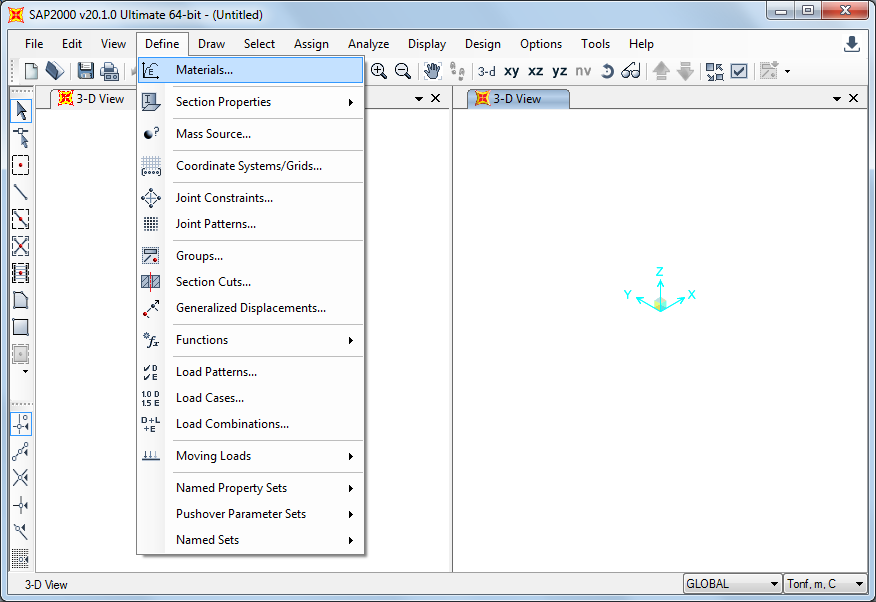
\includegraphics[width=1\textwidth]{metodologia/sap2000_toolbar.png}
%     \caption{Menús del programa de computador SAP2000\textsuperscript{\textregistered} para definir las características de la estructura.}
%     \label{fig:sap2000_toolbar}
% \end{figure}

% Una vez definidas las características de la estructura, el usuario procede a ingresar los diferentes elementos del modelo de la estructura en el entorno virtual de manera interactiva, mediante la ayuda de una serie de ejes y de los menús del programa. \\

% El entorno virtual consiste en un ambiente tridimensional donde el usuario puede ver, ingresar e interactuar con los diferentes elementos visuales del modelo.\\

% La serie de ejes consiste en un grupo de líneas en el espacio que se interceptan en un conjunto de puntos, los cuales sirven de referencia para que el usuario pueda ingresar los diferentes elementos del modelo al entorno virtual. En la figura \ref{fig:sap2000_axes} se presenta un conjunto de dichos ejes en el entorno virtual.\\
% \begin{figure}[ht]
%     \centering
%     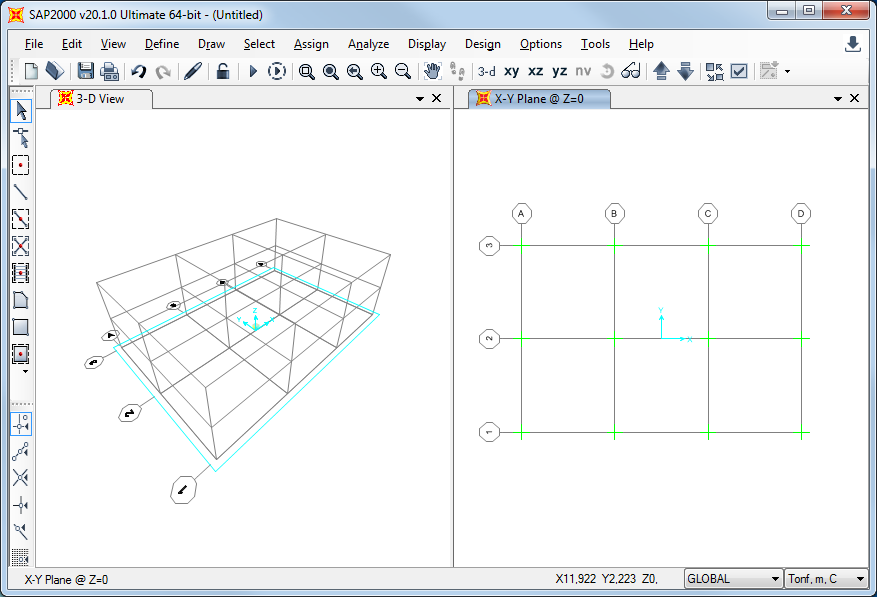
\includegraphics[width=1\textwidth]{metodologia/sap2000_axes.png}
%     \caption{Entorno virtual de SAP2000\textsuperscript{\textregistered} con un conjunto de ejes definido.}
%     \label{fig:sap2000_axes}
% \end{figure}

% Los menús del programa de computador que permiten ingresar los elementos del modelo consisten en aquellos que permiten escoger el tipo de elemento, como se muestra en la figura \ref{fig:sap200_draw}, y aquellos que permiten modificar los elementos ya ingresados, los cuales permiten moverlos, copiarlos, o eliminarlos. \\
% \begin{figure}[ht]
%     \centering
%     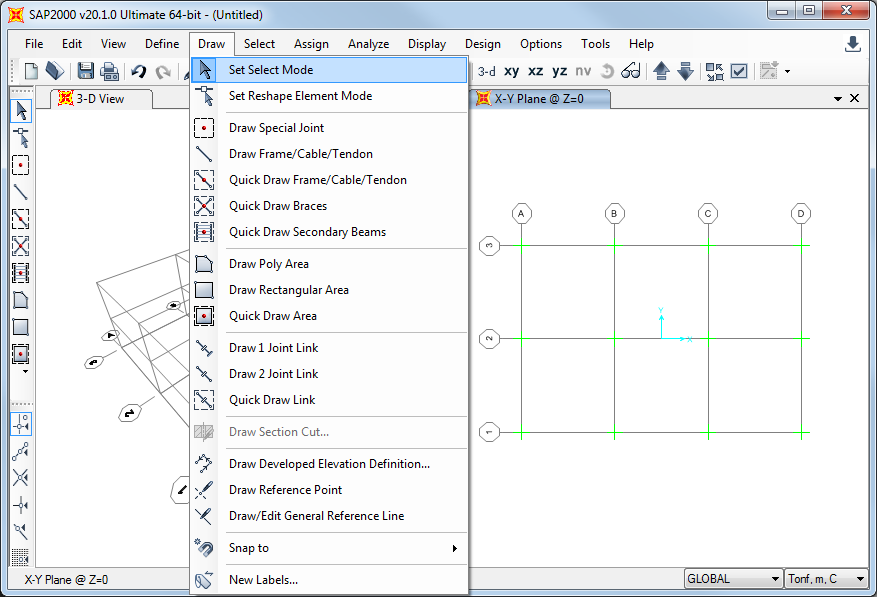
\includegraphics[width=1\textwidth]{metodologia/sap2000_draw.png}
%     \caption{Menú de SAP2000\textsuperscript{\textregistered} que permite ingresar diferentes tipos de elementos.}
%     \label{fig:sap200_draw}
% \end{figure}

% Una vez el usuario haya agregado los diferentes elementos de la estructura puede modificar sus condiciones de apoyo, las cargas, entre otros, mediante el uso de menús, de manera que el modelo esté listo para que el programa ejecute el análisis correspondiente. En la figura \ref{fig:sap2000_model} se presenta el modelo de una estructura terminado.
% \begin{figure}[ht]
%     \centering
%     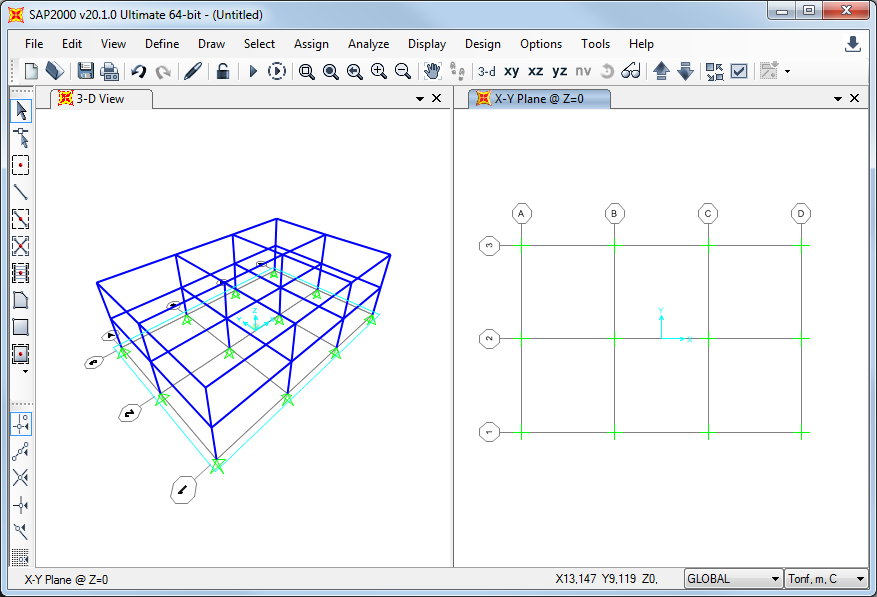
\includegraphics[width=1\textwidth]{metodologia/sap2000_model.png}
%     \caption{Modelo de una estructura en  SAP2000\textsuperscript{\textregistered}.}
%     \label{fig:sap2000_model}
% \end{figure}

% Una vez se han surtido los pasos anteriores, el usuario puede correr el análisis para obtener los resultados del mismo. El usuario puede visualizar los resultados en el entorno virtual, como se muestra en la figura \ref{fig:sap2000_deformed}, o mediante tablas.
% \begin{figure}[ht]
%     \centering
%     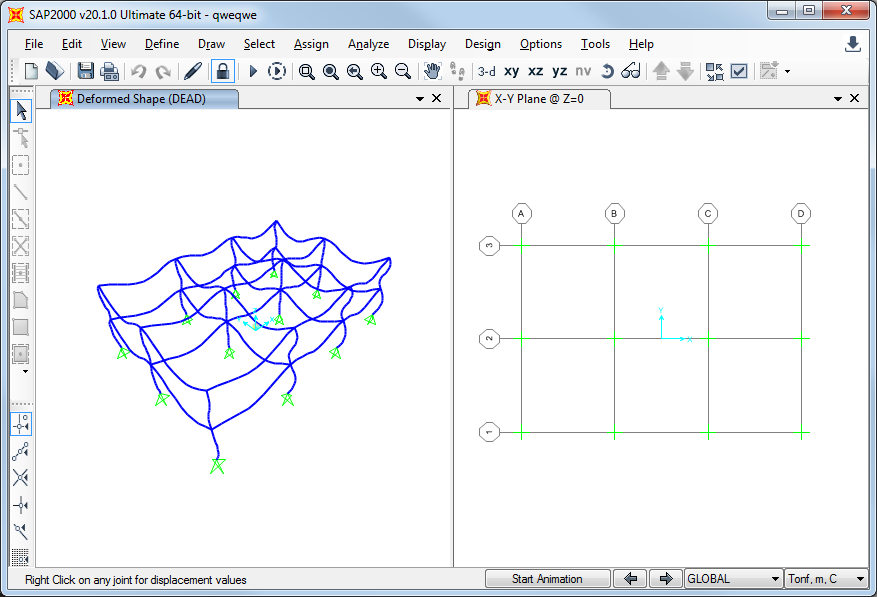
\includegraphics[width=1\textwidth]{metodologia/sap2000_deformed.png}
%     \caption{Deformación de la estructura después del análisis de SAP2000\textsuperscript{\textregistered}.}
%     \label{fig:sap2000_deformed}
% \end{figure}

% Así como el programa SAP2000\textsuperscript{\textregistered}, los otros programas comerciales, como ETABS \textsuperscript{\textregistered}, CSIBridge\textsuperscript{\textregistered}, midas\textsuperscript{\textregistered}, entre otros, cuentan con herramientas similares para que el usuario pueda analizar modelos de estructuras.

% \section{Revisión de los programas a código abierto}
% Existen gran variedad de programas a código abierto. Entre los programas que más se han estudiado para este trabajo se encuentra \textit{ANALEST}. \\

% El programa \textit{ANALEST} comprende una serie de subprogramas cuyo objeto es servir de ayuda en el análisis y diseño de estructuras. El programa está programado en \texttt{BASIC} y su característica principal es analizar 
% \begin{inparaenum}[$ (1) $]
%     \item vigas continúas, 
%     \item armaduras planas, 
%     \item armaduras en el espacio, 
%     \item pórticos planos, 
%     \item pórticos en el espacio, 
%     \item parrillas planas.
% \end{inparaenum}

% Para usar los subprogramas, se debe
% \begin{inparaenum}[$ (1) $]
%     \item introducir los datos del modelo de la estructura, revisarlos y guardarlos, 
%     \item introducir los datos de carga, revisarlos y guardarlos, 
%     \item ejecutar el análisis, guardar los resultados y presentarlos
% \end{inparaenum}

% Ademas, los subprogamas de vigas y armaduras permiten encontrar la envolvente de momentos en los apoyos y de fuerzas axiales, respectivamente, como paso preliminar para el diseño de los miembros. \\

% Guardar los datos estructurales y los datos de carga es muy útil en aquellos casos en que conviene modificar las dimensiones de los elementos con base en los resultados del primer análisis. Por otra parte, guardar los resultados facilita el estudio de las combinaciones de carga disminuyendo por una parte los datos requeridos y por otra el tiempo de ejecución, ya que se aprovecha el principio de superposición. Adicionalmente, guardar dichos resultados facilita el enlace de los subprogramas con programas de diseño, bien sean adquiridos o desarrollados por el usuario. \\

% \section{Identificación de los elementos a programar}

% De la revisión de los diferentes programas comerciales se dedujo que el programa StressUN debía dividirse en tres partes y que tenían que trabajar en conjunto. Dichas partes son: \textit{preproceso}, \textit{proceso} y \textit{posproceso}. \\

% El preproceso consiste en la adquisición de todos los datos relevantes del modelo de la estructura a analizar. El proceso realiza el tratamiento de los datos del modelo, mientras que el posproceso presenta los resultados del análisis del modelo. \\

% Tanto el preproceso como el posproceso necesitan de un ambiente gráfico, mientras que el proceso necesita de las rutinas propias del análisis matricial. \\

% \section{Selección de las herramientas de programación}
% Los dos grandes problemas a solucionar consistieron en desarrollar el ambiente gráfico, el cual se compone de menús y un entorno virtual tridimensional, y el núcleo de StressUN. Para esto, se consultó las diferentes herramientas de programación disponibles, donde se decidió utilizar la librería \textit{frames}, la cual está programada en el \textit{Java}, y el conjuto de librerías \textit{Scipy}, la cual está programada en \textit{Python}.\\

% La librería frames consiste en un conjunto de herramientas para crear un entorno virtual bidimensional o tridimensional interactivo. Dicha librería trabaja como una extensión de la librería \textit{processing}, la cual también está programada en Java. \\

% La librería processing es un conjunto de herramientas dirigida a solucionar los problemas relacionados con la computación gráfica, permitiendo a los desarrolladores desde crear imágenes hasta entornos virtuales tridimensionales. \\

% Por otro lado, el conjunto de librerías Scipy consiste en herramientas para solucionar problemas relacionados algebra matricial. Dicho conjunto de librerías está conformado por \textit{Numpy}, \textit{Scipy}, \textit{matplotlib}, entre otros. La librería Numpy provee arreglos multidimensionales y operaciones entre ellos. La librería \textit{Scipy} trata problemas del algebra matricial, como son la solución de sistemas de ecuaciones líneales, mientras que matplotlib permite generar diferentes tipos de gráficos. \\

% \section{Desarrollo del programa de computador}

% Una vez se identificaron los diferentes elementos necesarios con los que debía contar el programa de computador y se escogieron las herramientas de trabajo, se realizó una revisión bibliográfica de la formulación matemática de los métodos matriciales aplicados al análisis estructural, enfocada al análisis de estructuras tridimensionales de respuesta lineal. Adicionalmente, se realizó una revisión a la documentación de la librería frames.\\

% De dicho ejercicio se identificaron los datos de entrada que el usuario necesita definir y los datos de salida que espera obtener
% \begin{itemize}
%     \item \textit{Preproceso}
%     \begin{itemize}
%         \item Definición de los materiales.
%         \item Definición de las secciones transversales.
%         \item Definición de los nudos.
%         \item Definición de los elementos.
%         \item Definición de las condiciones de apoyo.
%         \item Definición de los casos de carga.
%         \item Definición de las combinaciones de carga.
%         \item Definición de las patrones de carga
%     \end{itemize}
%     \item \textit{Posproceso}
%     \begin{itemize}
%         \item Visualización de los desplazamientos en los nudos.
%         \item Visualización de las reacciones.
%         \item Visualización de las fuerzas internas.
%     \end{itemize}
    
% \end{itemize}

%  \textit{StressUN} se desarrolló usando el paradigma de \textit{programación orientada a objetos}, \textit{OOP} (de sus siglas en inglés \textit{object-oriented programming}), y en forma modular, de manera que el \textit{preproceso} y el \textit{posproceso} son independientes del \textit{proceso}.\\

% A medida que se definieron los diferentes elementos a tener en cuenta, se fueron programando. Es decir, se desarrollaron las clases \textit{primitivas} del programa, las cuales representan la abstracción de los elementos de las entidades más sencillas del problema, las cuales consisten en las clases
% \begin{itemize}
%     \item \textit{Material}.
%     \item \textit{Section}.
%     \item \textit{Node}.
%     \item \textit{Frame}.
%     \item \textit{Support}.
%     \item \textit{PointLoad}.
%     \item \textit{LoadPattern}.
%     \item \textit{Displacement}.
% \end{itemize}

% Las clases anteriormente listadas, tienen su representación tanto en el preproceso y posproceso, como en el proceso. Es decir, en el preproceso y posproceso dichas clases tienen su representación gráfica, mientras que en el proceso, éstos tienen su representación matemática. Sin embargo, dichas clases son separadas unas de las otras, de manera que se asegure que el preproceso y posproceso son independientes del proceso.

% Una vez programados las entidades más básicas del programa, se procedió a crear la clase \textit{Structure}, la cual se encarga de administrar otros objetos. Dicho paradigma de programación se conoce como \textit{composición}. Los objetos que contiene la clase \textit{Structure} son

% \begin{itemize}
%     \item \textit{Materials}.
%     \item \textit{Sections}.
%     \item \textit{Nodes}.
%     \item \textit{Frames}.
%     \item \textit{Supports}.
%     \item \textit{LoadPatterns}.
% \end{itemize}

% Cada una de las anteriores clases es la interfaz entre el programa y el usuario, donde este último podrá agregar nuevos materiales, secciones, nudos, elementos tipo pórtico, condiciones de apoyo y condiciones de carga. Dichas clases componen el \textit{núcleo} del programa.\\

% El proceso anteriormente descrito se desarrolló bajo los diferentes mecanismos que provee la programación orientada objeto, los cuales son encapsulación, herencia y sobre carga. Estas herramientas, bien aplicadas, permiten la reutilización del código y el mantenimiento del mismo. Así mismo, se utilizó la herramienta de \textit{Git}, la cual es un sistema de control de versiones, la cual permite llevar el control absoluto durante el proceso de desarrollo del código.\\

% \section{Verificación del programa}

% Una vez se llegó a una versión estable del programa, este se puso a prueba mediante la solución de diferentes problemas que aparecen en la bibliografía, donde se comparó la respuesta obtenida con la presentada. Así mismo, se comparó el desempeño del programa frente a otros programas, tanto comerciales como académicos, en cuanto a la facilidad de uso como al tiempo de computo. \\